\begin{figure}
	\centering
	\begin{subfigure}{.45\textwidth}
		\centering
		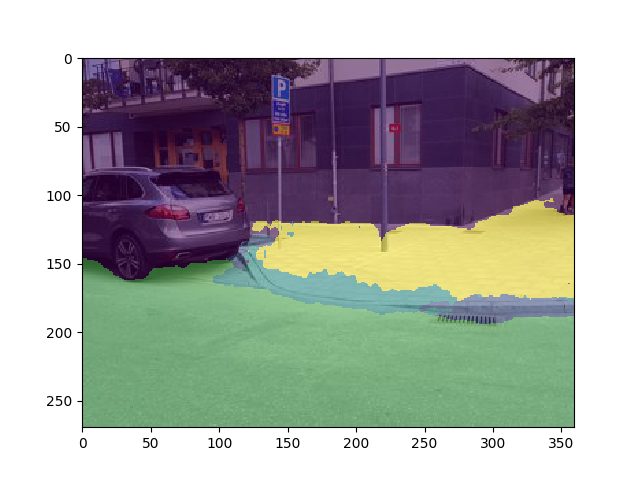
\includegraphics[width=\linewidth]{figures/experiments/results-mapillary/1.png}
		\caption[Mapillary Vistas Segmentation Result 1]{}
		\label{fig:mapresult-1}
	\end{subfigure}
	\hfill
	\begin{subfigure}{.45\textwidth}
		\centering
		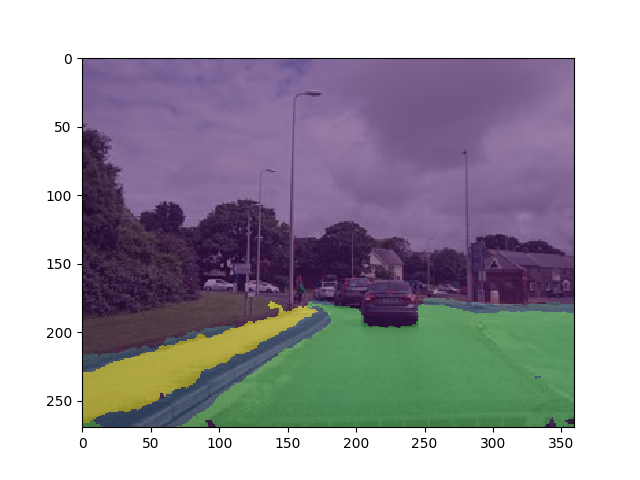
\includegraphics[width=\linewidth]{figures/experiments/results-mapillary/2.png}
		\caption[Mapillary Vistas Segmentation Result 2]{}
		\label{fig:mapresult-2}
	\end{subfigure}
	
	\vspace{12pt}%------------
	
	\begin{subfigure}{.45\textwidth}
		\centering
		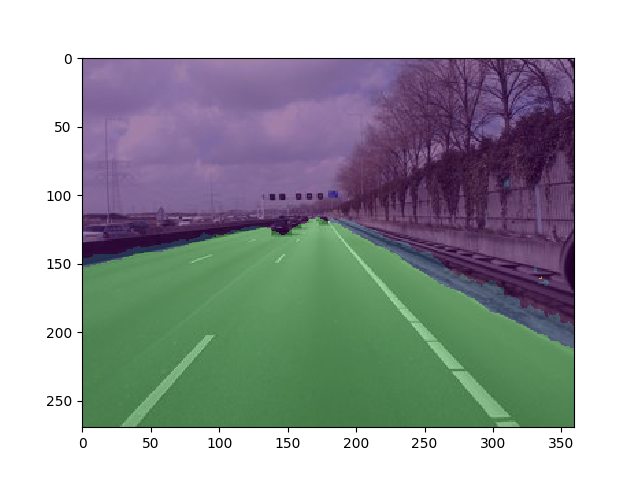
\includegraphics[width=\linewidth]{figures/experiments/results-mapillary/3.png}
		\caption[Mapillary Vistas Segmentation Result 3]{}
		\label{fig:mapresult-3}
	\end{subfigure}
	\hfill
	\begin{subfigure}{.45\textwidth}
		\centering
		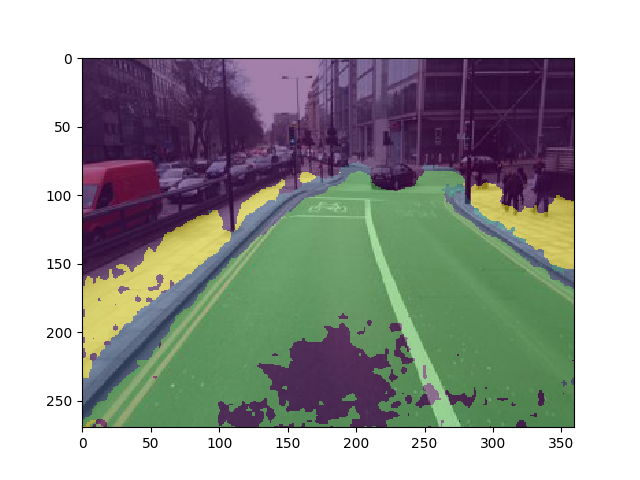
\includegraphics[width=\linewidth]{figures/experiments/results-mapillary/4.png}
		\caption[Mapillary Vistas Segmentation Result 4]{}
		\label{fig:mapresult-4}
	\end{subfigure}

	\vspace{12pt}%------------
	
	\begin{subfigure}{.45\textwidth}
		\centering
		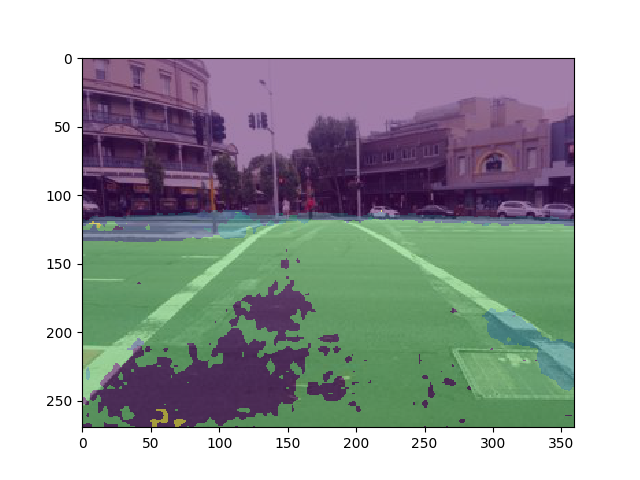
\includegraphics[width=\linewidth]{figures/experiments/results-mapillary/5.png}
		\caption[Mapillary Vistas Segmentation Result 5]{}
		\label{fig:mapresult-5}
	\end{subfigure}
	\hfill
	\begin{subfigure}{.45\textwidth}
		\centering
		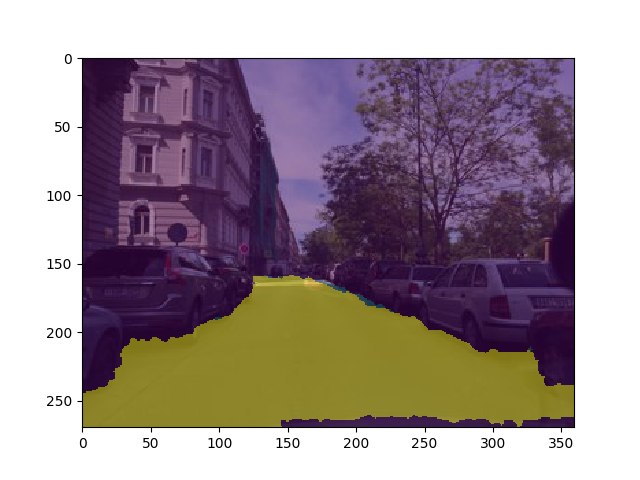
\includegraphics[width=\linewidth]{figures/experiments/results-mapillary/6.png}
		\caption[Mapillary Vistas Segmentation Result 6]{}
		\label{fig:mapresult-6}
	\end{subfigure}

	\caption[Mapillary Vistas Segmentation Results]{A sample of some segmentation results from the trained CurbNet model. The images are from the Mapillary Vistas dataset \cite{mapillary}. Green is road, yellow is sidewalk, blue is curb, turquoise is curb cuts, and purple is the ignore class. Figure \ref{fig:mapresult-1} shows how the model is able to identify all of the different traversibility classes. Figures \ref{fig:mapresult-2} and \ref{fig:mapresult-3} shows that segmentation of curbs even in the distance can be performed well. Figures \ref{fig:mapresult-4} and \ref{fig:mapresult-5} shows that curb cuts in the distance are also identified and segmented by the network, although sometimes roads are mislabeled as ignore. Figure \ref{fig:mapresult-5} also shows a failure case where some road markings in the bottom right corner have been mislabeled as curb. Figure \ref{fig:mapresult-6} shows a case where the entire road is labeled as sidewalk.}
	\label{fig:experiments-resultsmapillary}
\end{figure}